\documentclass[12pt, letterpaper, onecolumn]{article}
\usepackage[utf8]{inputenc}
\usepackage[english]{babel}
\usepackage{pdfpages}
\usepackage{amssymb}
\usepackage{graphicx}
\usepackage{setspace}
\usepackage{nicefrac}
\usepackage{hyperref}
\usepackage{pgfplots}
\usepackage{grffile}
\usepackage{amsmath}
\usepackage{commath}
\usepackage{siunitx}
\usepackage{float}

\pgfplotsset{compat=newest}
\usetikzlibrary{plotmarks}
\usetikzlibrary{arrows.meta}
\usepgfplotslibrary{patchplots}
\NewDocumentCommand{\codeword}{v}{% 
\texttt{#1}}%
\DeclareMathOperator{\Span}{span}

\title{Project 1 - MECH 7790}
\author{Andrew Weir, Tanner Koza}
\date\today

\begin{document}
\maketitle

\section*{Part 1: Develop the LTI Model}

\subsection*{Problem 1}
The following depicts the system model rewritten in the desired form:

\begin{equation*}
    \begin{split}
        \begin{bmatrix}
            M+m            & ml\cos(\theta) \\
            ml\cos(\theta) & I+ml^2         \\
        \end{bmatrix}
        \begin{bmatrix}
            \ddot{x}      \\
            \ddot{\theta} \\
        \end{bmatrix}
        & =
        \begin{bmatrix}
            F + ml{\dot{\theta}}^2\sin(\theta)-b\dot{x} \\
            -mgl\sin(\theta)
        \end{bmatrix}
    \end{split}
\end{equation*}

\subsection*{Problem 2}
The following depicts the solution for $\ddot{x}$ and $\ddot{\theta}$:


\begin{equation*}
    \begin{split}
        \ddot{x} & = \frac{F\,\textrm{I}-\textrm{I}\,b\,\dot{x} +F\,l^2 \,m-b\,l^2 \,m\,\dot{x} +l^3 \,m^2 \,{\dot{\theta} }^2 \,\sin \left(\theta \right)+g\,l^2 \,m^2 \,\cos \left(\theta \right)\,\sin \left(\theta \right)+\textrm{I}\,l\,m\,{\dot{\theta} }^2 \,\sin \left(\theta \right)}{-l^2 \,m^2 \,{\cos \left(\theta \right)}^2 +l^2 \,m^2 +M\,l^2 \,m+\textrm{I}\,m+\textrm{I}\,M} \\
        \ddot{\theta} & = -\frac{l\,m\,{\left(l\,m\,\cos \left(\theta \right)\,\sin \left(\theta \right)\,{\dot{\theta} }^2 +F\,\cos \left(\theta \right)-b\,\dot{x} \,\cos \left(\theta \right)+g\,m\,\sin \left(\theta \right)+M\,g\,\sin \left(\theta \right)\right)}}{-l^2 \,m^2 \,{\cos \left(\theta \right)}^2 +l^2 \,m^2 +M\,l^2 \,m+\textrm{I}\,m+\textrm{I}\,M}
    \end{split}
\end{equation*}

\subsection*{Problem 3}
The following depicts the system model in the form $\dot{z} = f(z,u)$ after using the relationship $\cos(\theta) = -\cos(\phi)$:

\begin{equation*}
    \begin{split}
        \dot{z} & =
        \begin{bmatrix}
            \dot{z_1} \\
            \dot{z_2} \\
            \dot{z_3} \\
            \dot{z_4} \\
        \end{bmatrix} \\
    \end{split}
\end{equation*}

\begin{equation*}
    \begin{split}
        & =
        \begin{bmatrix}
            \dot{x}                                                                                                                                                                                                                                                                                                                                                      \\
            -\frac{\textrm{I}\,b\,\dot{x} -F\,\textrm{I}-F\,l^2 \,m+b\,l^2 \,m\,\dot{x} +l^3 \,m^2 \,{\dot{\phi} }^2 \,\sin \left(\phi \right)-g\,l^2 \,m^2 \,\cos \left(\phi \right)\,\sin \left(\phi \right)+\textrm{I}\,l\,m\,{\dot{\phi} }^2 \,\sin \left(\phi \right)}{-l^2 \,m^2 \,{\cos \left(\phi \right)}^2 +l^2 \,m^2 +M\,l^2 \,m+\textrm{I}\,m+\textrm{I}\,M} \\
            \dot{\phi}                                                                                                                                                                                                                                                                                                                                                   \\
            \frac{l\,m\,{\left(-l\,m\,\cos \left(\phi \right)\,\sin \left(\phi \right)\,{\dot{\phi} }^2 +F\,\cos \left(\phi \right)-b\,\dot{x} \,\cos \left(\phi \right)+g\,m\,\sin \left(\phi \right)+M\,g\,\sin \left(\phi \right)\right)}}{-l^2 \,m^2 \,{\cos \left(\phi \right)}^2 +l^2 \,m^2 +M\,l^2 \,m+\textrm{I}\,m+\textrm{I}\,M}                               \\
        \end{bmatrix} \\
        & =
        \begin{bmatrix}
            z_2                                                                                                                                                                                                                                                                                                                               \\
            -\frac{\textrm{I}\,b\,z_2 -F\,\textrm{I}-F\,l^2 \,m+b\,l^2 \,m\,z_2 +l^3 \,m^2 \,{z_4 }^2 \,\sin \left(z_3 \right)-g\,l^2 \,m^2 \,\cos \left(z_3 \right)\,\sin \left(z_3 \right)+\textrm{I}\,l\,m\,{z_4 }^2 \,\sin \left(z_3 \right)}{-l^2 \,m^2 \,{\cos \left(z_3 \right)}^2 +l^2 \,m^2 +M\,l^2 \,m+\textrm{I}\,m+\textrm{I}\,M} \\
            z_4                                                                                                                                                                                                                                                                                                                               \\
            \frac{l\,m\,{\left(-l\,m\,\cos \left(z_3 \right)\,\sin \left(z_3 \right)\,{z_4 }^2 +F\,\cos \left(z_3 \right)-b\,z_2 \,\cos \left(z_3 \right)+g\,m\,\sin \left(z_3 \right)+M\,g\,\sin \left(z_3 \right)\right)}}{-l^2 \,m^2 \,{\cos \left(z_3 \right)}^2 +l^2 \,m^2 +M\,l^2 \,m+\textrm{I}\,m+\textrm{I}\,M}                      \\
        \end{bmatrix} \\
    \end{split}
\end{equation*}

\subsection*{Problem 4}
\subsubsection*{a) Determine $z^{eq}$ and $u^{eq}$.}
Given $z_1^{eq}, z_3^{eq} = 0$, $z_2^{eq}$ and $z_4^{eq}$ are also 0 as they are the derivatives of $z$ states 1 and 3 ($x$ and $\phi$). Therefore, $z^{eq}$ is the following:

\begin{equation*}
    \begin{split}
        z^{eq} & =
        \begin{bmatrix}
            0 \\
            0 \\
            0 \\
            0 \\
        \end{bmatrix}
    \end{split}
\end{equation*}

Given $z^{eq}$ is 0, evaluating the system model at equilibrium subsequently makes $u^{eq}$ equal to 0.


\subsubsection*{b) Write out the linearized state space matrices for the model.}
Evaluating the partial derivatives $\frac{\partial f}{\partial z_{1-4}},\frac{\partial f}{\partial u},\frac{\partial g}{\partial z_{1-4}},\frac{\partial g}{\partial u}$ at the equilibrium points yields the following system state space matrices:

\begin{equation*}
    \begin{split}
        A & =
        \begin{bmatrix}
            0 & 1                               & 0                             & 0 \\
            0 & \frac{-b(I+ml^2)}{I(M+m)+Mml^2} & \frac{m^2gl^2}{I(M+m)+Mml^2}  & 0 \\
            0 & 0                               & 0                             & 1 \\
            0 & \frac{-mlb}{I(M+m)+Mml^2}       & \frac{mgl(M+m)}{I(M+m)+Mml^2} & 0 \\
        \end{bmatrix} \\
        B & =
        \begin{bmatrix}
            0                           \\
            \frac{I+ml^2}{I(M+m)+Mml^2} \\
            0                           \\
            \frac{ml}{I(M+m)+Mml^2}
        \end{bmatrix} \\
        C & =
        \begin{bmatrix}
            1 & 0 & 0 & 0 \\
            0 & 0 & 1 & 0 \\
        \end{bmatrix} \\
        D & =
        \begin{bmatrix}
            0 \\
            0 \\
        \end{bmatrix} \\
    \end{split}
\end{equation*}

\subsubsection*{c) Substitute in numeric values for matrices.}
Using the property values given in the assignment, the system state space matrices equate to the following:

\begin{equation*}
    \begin{split}
        A & =
        \begin{bmatrix}
            0 & 1       & 0       & 0 \\
            0 & -0.1818 & 2.6727  & 0 \\
            0 & 0       & 0       & 1 \\
            0 & -0.4545 & 31.1818 & 0 \\
        \end{bmatrix} \\
        B & =
        \begin{bmatrix}
            0      \\
            1.8182 \\
            0      \\
            4.5455 \\
        \end{bmatrix} \\
        C & =
        \begin{bmatrix}
            1 & 0 & 0 & 0 \\
            0 & 0 & 1 & 0 \\
        \end{bmatrix} \\
        D & =
        \begin{bmatrix}
            0 \\
            0 \\
        \end{bmatrix} \\
    \end{split}
\end{equation*}


\clearpage

\section*{Part 2: Linear Model Properties}

\subsection*{Problem 1}
The eigenvalues of the open-loop system were determined using \codeword{eig()} in MATLAB\@. It was determined $s=0, -0.1428,-5.6041,$ and $5.5651$. These eigenvalues (or poles) indicate the open-loop system is unstable because of the eigenvalue $s=5.5651$.
\subsection*{Problem 2}
The eigenvectors of the open-loop system were also determined using \codeword{eig()} in MATLAB\@. They are as presented in the columns of the following matrix:

\begin{equation*}
    \begin{split}
        V_{OL} & =
        \begin{bmatrix}
            1 & -0.9899 & -0.0154 & 0.0147 \\
            0 & 0.1414  & 0.0863  & 0.0819 \\
            0 & 0.0021  & -0.1749 & 0.1762 \\
            0 & -0.0003 & 0.9807  & 0.9808 \\
        \end{bmatrix}
    \end{split}
\end{equation*}

The stable subspace of the open-loop system is given by columns 1-3. Specifically, the $span\{V_{OL(:,1:3)}\}$. On the other hand, the  $span\{V_{OL(:,4)}\}$ describes the unstable subspace.

\subsection*{Problem 3}
Given the linear model is unstable, it can be assumed the nonlinear model is as well.
\subsection*{Problem 4}
The controllability was determined by evaluating the rank of the controllability matrix that was found using \codeword{ctrb()} in MATLAB\@. The controllability matrix was determined to be the following:


\begin{equation*}
    \begin{split}
        CO & =
        \begin{bmatrix}
            0      & 1.8182   & -0.33058 & 12.221  \\
            1.8182 & -0.33058 & 12.221   & -4.4332 \\
            0      & 4.5455   & -0.82645 & 142.03  \\
            4.5455 & -0.82645 & 142.03   & -31.352 \\
        \end{bmatrix}
    \end{split}
\end{equation*}

This matrix $CO$ is full rank, therefore the system is controllable. The stabilizability was determined by finding the rank of the augmented matrix

\begin{equation*}
    \begin{split}
        SB & =
        \begin{bmatrix}
            D-A & B \\
        \end{bmatrix}
    \end{split}
\end{equation*}

where $D$ is the diagonal matrix of open-loop eigenvalues. This matrix is also full rank meaning the system is stabilizable, although this is inherently true when controllable.

\subsection*{Problem 5}
The observability was determined by evaluating the rank of the observability matrix that was found using \codeword{obsv()} in MATLAB\@. The observability matrix was determined to be the following:


\begin{equation*}
    \begin{split}
        OB & =
        \begin{bmatrix}
            1 & 0        & 0        & 0      \\
            0 & 0        & 1        & 0      \\
            0 & 1        & 0        & 0      \\
            0 & 0        & 0        & 1      \\
            0 & -0.18182 & 2.6755   & 0      \\
            0 & -0.45455 & 31.214   & 0      \\
            0 & 0.033058 & -0.48645 & 2.6755 \\
            0 & 0.082645 & -1.2161  & 31.214 \\
        \end{bmatrix}
    \end{split}
\end{equation*}

This matrix $OB$ is full rank, therefore the system is observable. The detectability was determined by finding the rank of the augmented matrix

\begin{equation*}
    \begin{split}
        SB & =
        \begin{bmatrix}
            D-A \\
            C   \\
        \end{bmatrix}
    \end{split}
\end{equation*}

where $D$ is the diagonal matrix of open-loop eigenvalues. This matrix is also full rank meaning the system is detectable, although this is inherently true when observable.

\subsection*{Problem 6}
This realization of the system was determined to be minimal using the \codeword{minreal()} function in MATLAB\@. The system state space matrices that were returned by this function matched the input, leading us to this conclusion.

\subsection*{Problem 7}
The transfer functions for this state space system were calculated using \codeword{ss2tf()} in MATLAB\@. They are as follows:

\begin{equation*}
    \begin{split}
        \frac{x}{u} & = \frac{1.818s^2 - 44.58}{s^4 - 0.1818s^3 -31.21s^2 -4.459s} \\
        \frac{\phi}{u} & = \frac{1.818s}{s^3 - 0.1818s^2 -31.21s -4.459}
    \end{split}
\end{equation*}

\clearpage

\section*{Part 3: State Feedback Regulation}

\subsection*{Problem 1}
\subsubsection*{a) Design the controller for the linear model.}
Given the design requirements, the poles for pole placement were chosen using the following method:

\begin{equation*}
    \begin{split}
        T_S & = 5 s \\
        \zeta\omega_n & = 4/T_S = 0.8 \\
    \end{split}
\end{equation*}

Two arbitrary damping coefficients ($\zeta$) were chosen to provide two sets of complex conjugate eigenvalues for the determination of the controller gains $K$.

\begin{equation*}
    \begin{split}
        \zeta_1 & = 0.2 \\
        \zeta_2 & = 0.4 \\
    \end{split}
\end{equation*}

The complex conjugate eigenvalue pairs were determined by finding the roots of $s^2 +2\zeta\omega_n +\omega_n^2$. This characteristic equation forms a good basis for the tuning even though our system is higher order. The closed-loop eigenvalues were determined to be the following:

\begin{equation*}
    \begin{split}
        s & = -0.8\pm 3.92i, -0.8\pm1.83i
    \end{split}
\end{equation*}

To account for the higher-order dynamics, the real components of the eigenvalues were shifted left in the complex plane by an arbitrary 1.5. This allowed us to comfortably meet the design requirements. The new eigenvalues are as follows:

\begin{equation*}
    \begin{split}
        s & = -2.3\pm 3.92i, -2.3\pm1.83i
    \end{split}
\end{equation*}

Using \codeword{place()} in MATLAB, we were able to obtain the following control matrix:

\begin{equation*}
    \begin{split}
        K & =
        \begin{bmatrix}
            -4.0058 & -3.1226 & 19.571 & 3.233 \\
        \end{bmatrix}
    \end{split}
\end{equation*}

The corresponding output and input plots are shown below:

\begin{figure}[h!]
    \centering
    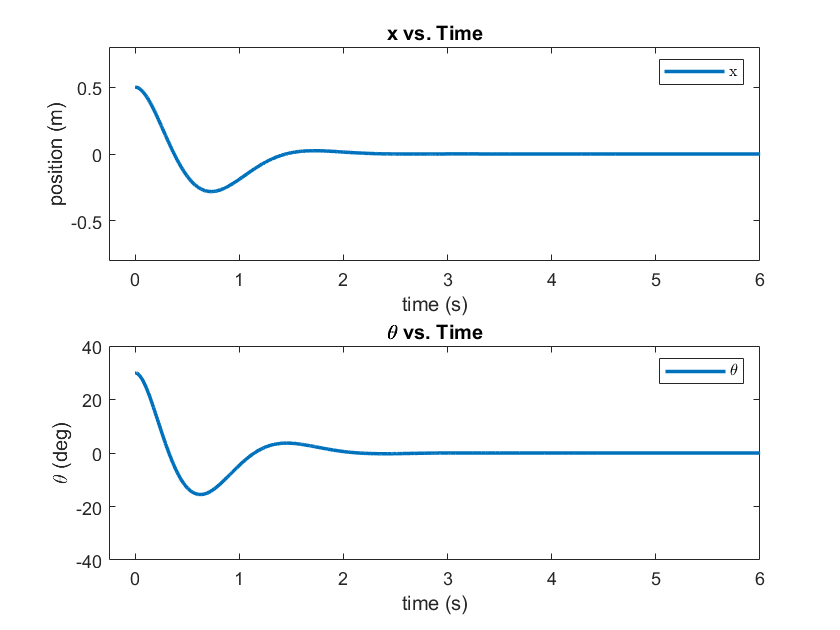
\includegraphics[width=\linewidth]{figs/p3-a-states.png}
    \caption{Linear Model: States vs. Time}
    \label{}
\end{figure}

\begin{figure}[h!]
    \centering
    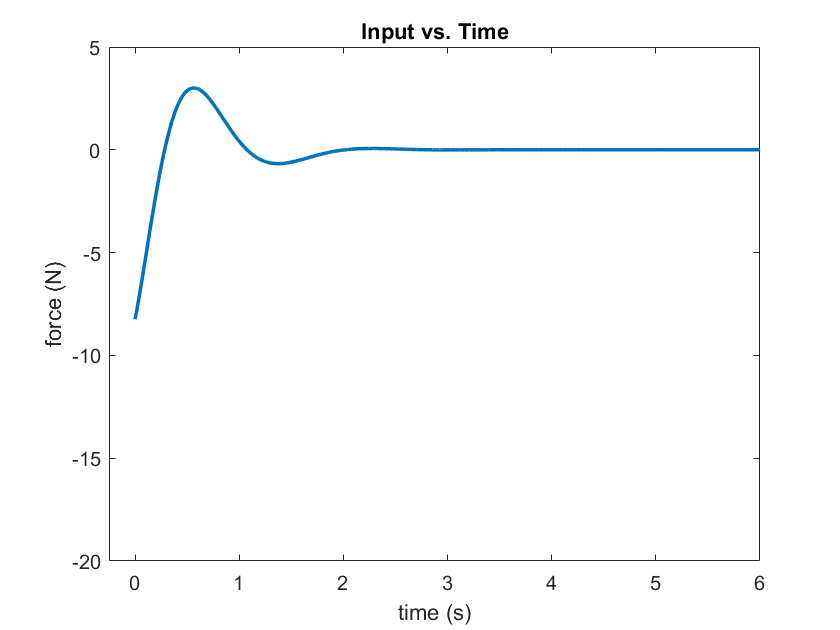
\includegraphics[width=\linewidth]{figs/p3-a-input.png}
    \caption{Linear Model: Control Effort vs. Time}
    \label{}
\end{figure}

\clearpage

\subsubsection*{b) Design the controller for the nonlinear model.}
The same controller used for the linear model was used for the nonlinear model as the arbitrary eigenvalue adjustment for the design requirements is enough to compensate for the nonlinearities. The $K$ matrix is the same as above. The output and input plots are shown below:

\begin{figure}[h!]
    \centering
    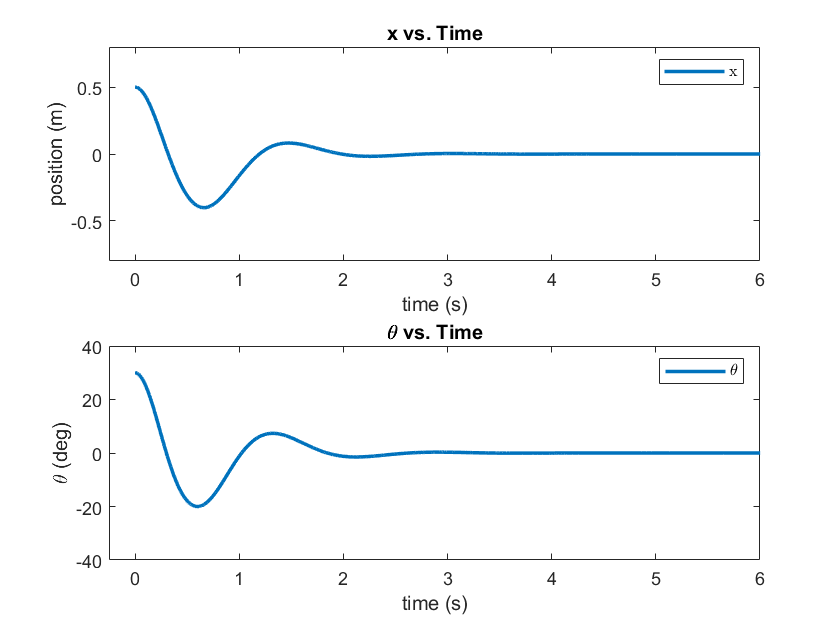
\includegraphics[width=\linewidth]{figs/p3-b-states.png}
    \caption{Nonlinear Model: States vs. Time}
    \label{}
\end{figure}

\begin{figure}[h!]
    \centering
    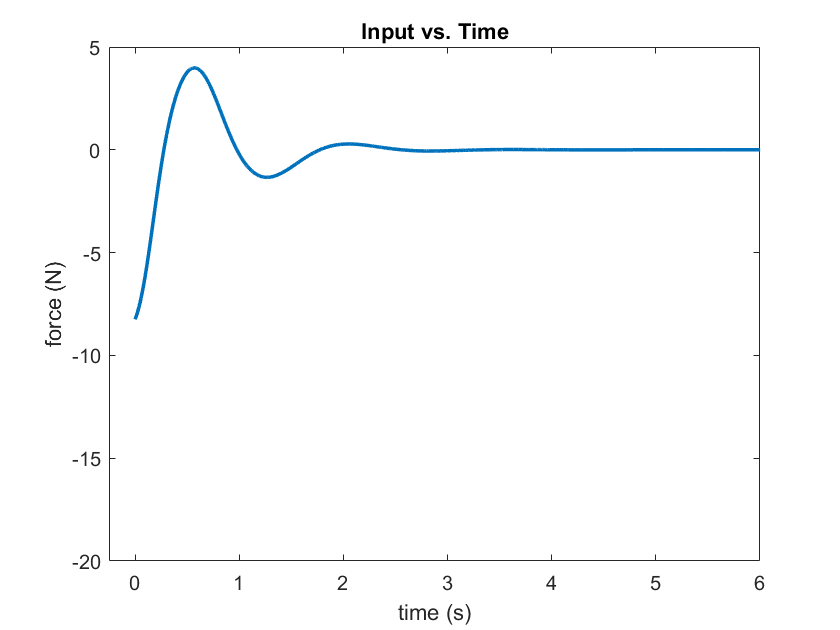
\includegraphics[width=\linewidth]{figs/p3-b-input.png}
    \caption{Nonlinear Model: Input vs. Time}
    \label{}
\end{figure}

\clearpage

\subsubsection*{c) Discuss differences in tuning for the linear and nonlinear model.}
In our case, there were no differences in tuning because we initially chose the eigenvalues to provide some design requirement buffer. It just so happens that this buffer was enough to compensate for the unaccounted dynamics in the nonlinear model. We understand that the available range of eigenvalues that meet the design requirements is limited by the nonlinearities when compared to the linear model. The effects of these unaccounted dynamics can be seen in the slower steady-state time of the nonlinear response. However, this time is still within the requirements. Also, our responses display the $\theta$ value of the response as this is the value we're considering for our design requirements. The max value seen for each of these responses was less than 32 degrees, meeting our design requirement.

\clearpage

\section*{Part 4: State Feedback Setpoint Tracking}

\subsection*{Problem 1}
The following relationship is used to only drive $z_1$ to a reference:

\begin{equation*}
    \begin{split}
        z_1 & = \bar{C}z
    \end{split}
\end{equation*}

Given we are only trying to control $x$ to a reference other than 0,the following augmented $A$ and $B$ matrices are used:

\begin{equation*}
    \begin{split}
        \bar{A} & =
        \begin{bmatrix}
            A       & 0 \\
            \bar{C} & 0 \\
        \end{bmatrix} \\
        \bar{B} & =
        \begin{bmatrix}
            B \\
            0 \\
        \end{bmatrix}
    \end{split}
\end{equation*}

where $\bar{C}$ is the following:

\begin{equation*}
    \begin{split}
        \bar{C} & =
        \begin{bmatrix}
            1 & 0 & 0 & 0 \\
        \end{bmatrix}
    \end{split}
\end{equation*}

The rank of the resulting controllability matrix is 5 and, therefore, full. $\bar{A}$'s new states now include the original $z$ states and an integrated error term. This yields a new $K$:

\begin{equation*}
    \begin{split}
        K & =
        \begin{bmatrix}
            -10.958 & -6.101 & 27.007 & 4.9304 & -9.213 \\
        \end{bmatrix}
    \end{split}
\end{equation*}

where the last term controls the integrated error. The eigenvalues for this system are the same as in Part 3 with an added eigenvalue of -2.3 for the fifth state to replicate the real components of the other eigenvalues. \\

\clearpage

The output and input plots for the controller are shown below:

\begin{figure}[!h]
    \centering
    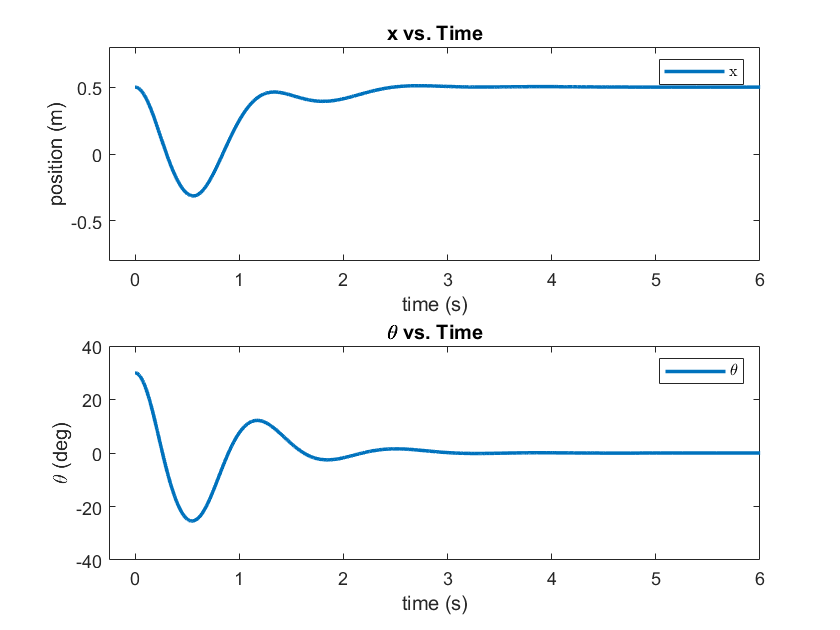
\includegraphics[width=\linewidth]{figs/p4-a-states.png}
    \caption{Nonlinear Model: States vs. Time}
    \label{}
\end{figure}

\begin{figure}[!h]
    \centering
    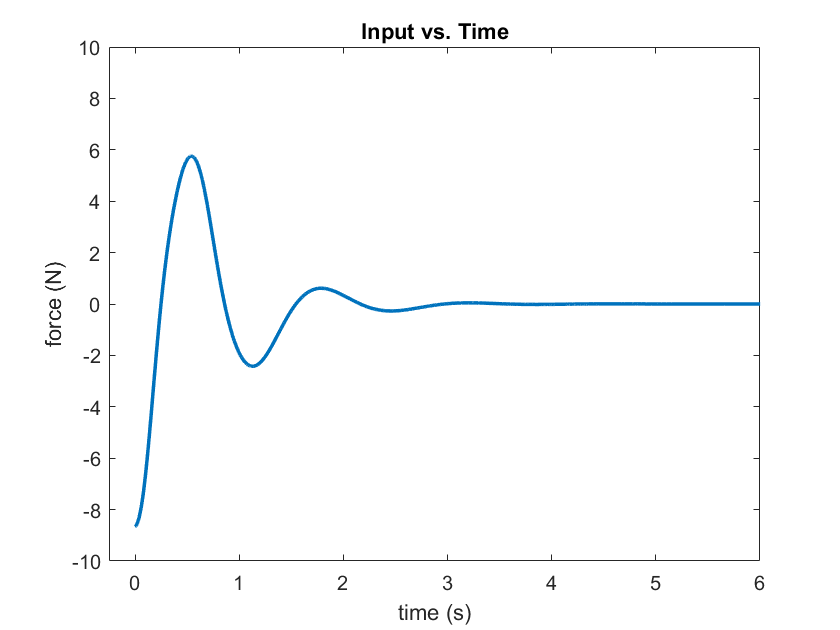
\includegraphics[width=\linewidth]{figs/p4-a-input.png}
    \caption{Nonlinear Model: Control Effort vs. Time}
    \label{}
\end{figure}

\clearpage

\section*{Part 5: Output Feedback Regulation (Full-Order)}

\subsection*{Problem 1}
\subsubsection*{a) Design the observer for the linear model and use the control matrix from Part 3.}
The observer was designed much like the controller in Part 3. Its eigenvalues were set to be an arbitrary 7.5 times greater in magnitude than the controller eigenvalues so the estimate of the states would converge faster than the states themselves. The eigenvalues are as follows:

\begin{equation*}
    \begin{split}
        s & = -17.25\pm 29.39i, -17.25\pm13.75i
    \end{split}
\end{equation*}

\codeword{place()} was used again with the $A$ and $C$ matrix to determine the observer matrix:

\begin{equation*}
    \begin{split}
        L & =
        \begin{bmatrix}
            34.214  & 15.885 \\
            681.48  & 260.8  \\
            -15.816 & 34.605 \\
            -293.28 & 740.41 \\
        \end{bmatrix}
    \end{split}
\end{equation*}

It can be seen that the design requirements are still met. The plots of the output and input follow:

\begin{figure}[!h]
    \centering
    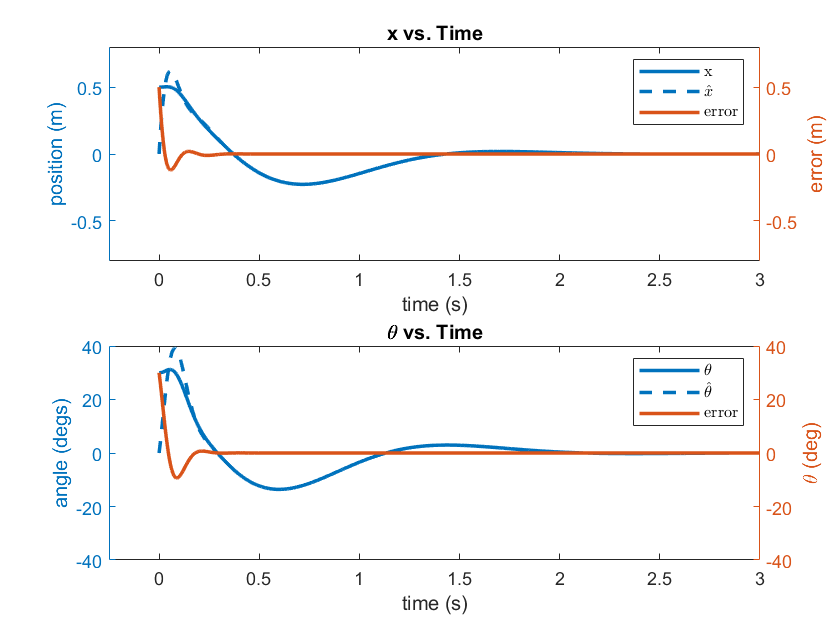
\includegraphics[width=\linewidth]{figs/p5-a-states.png}
    \caption{Linear Model: States \& Error vs. Time}
    \label{}
\end{figure}

\begin{figure}[!h]
    \centering
    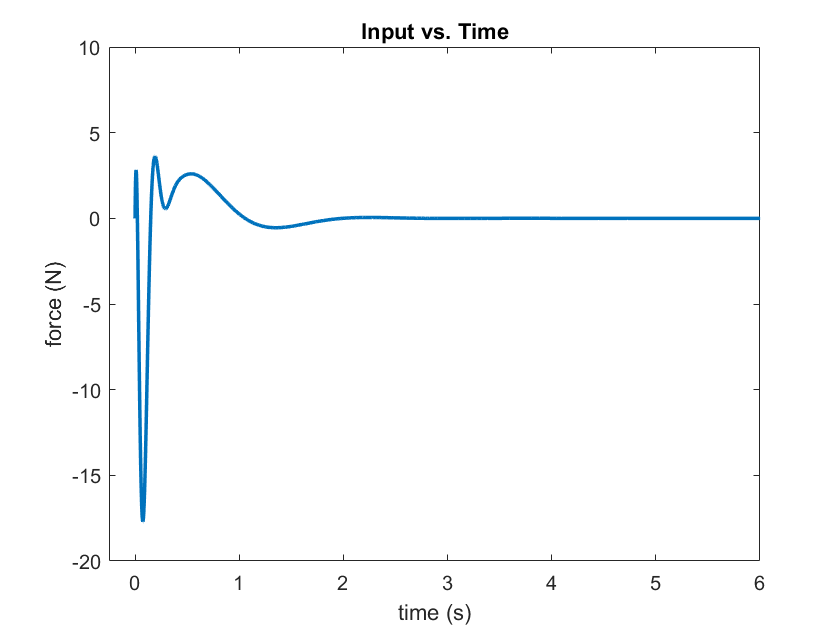
\includegraphics[width=\linewidth]{figs/p5-a-inputs.png}
    \caption{Linear Model: Control Effort vs. Time}
    \label{}
\end{figure}

\clearpage

\subsubsection*{b) Determine the observer matrix and the controller matrix for the nonlinear model.}
The $L$ and $K$ for the nonlinear model are the same as the linear model. Like in Part 3, the chosen eigenvalues of the observer and controller were given enough of a buffer to handle the un-modeled dynamics. Refer to Part 3.a and Part 5.a, for the eigenvalues used for the nonlinear model. The plots of the output and input follow:

\begin{figure}[!h]
    \centering
    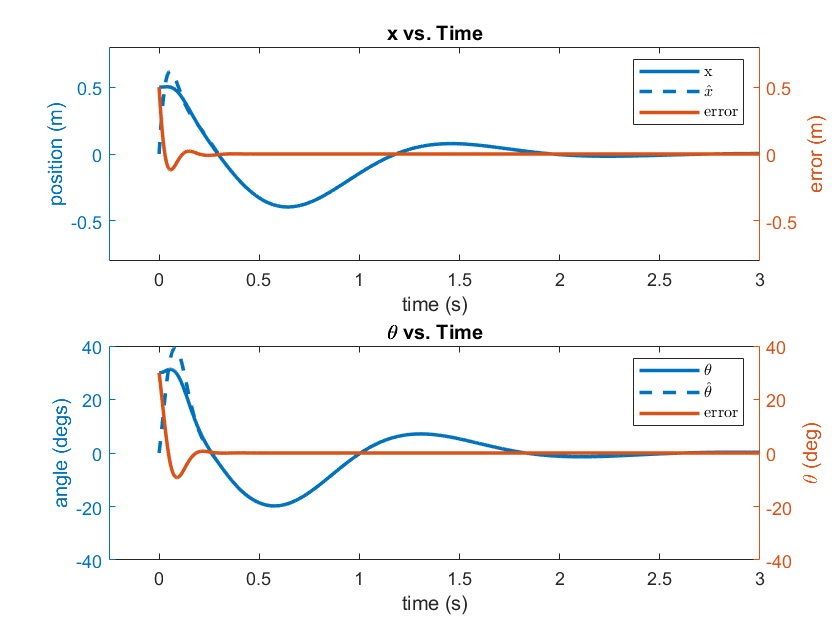
\includegraphics[width=\linewidth]{figs/p5-b-states.png}
    \caption{Nonlinear Model: States \& Error vs. Time}
    \label{}
\end{figure}

\begin{figure}[!h]
    \centering
    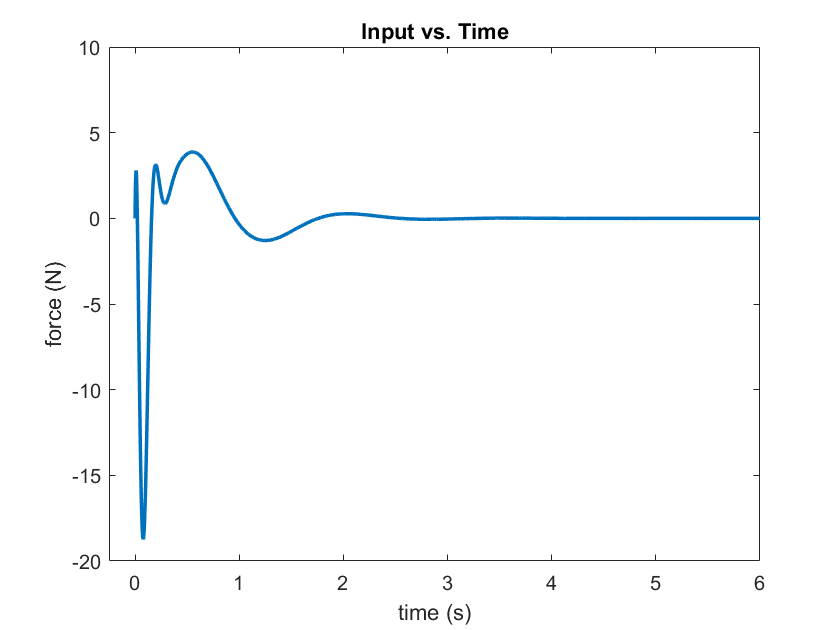
\includegraphics[width=\linewidth]{figs/p5-b-input.png}
    \caption{Nonlinear Model: Control Effort vs. Time}
    \label{}
\end{figure}

\clearpage

The primary difference between the control of these two models can be seen in the marginally slower response time for the nonlinear case and, primarily, the difference in control effort during the transient period of control. On the other hand, the observer response looks the same. The output and input plots for when $\codeword{eig(A-LC)} = \codeword{eig(A-BK)} = -0.8\pm 3.92i, -0.8\pm1.83i$ are shown below for the linear and nonlinear case:

\begin{figure}[!h]
    \centering
    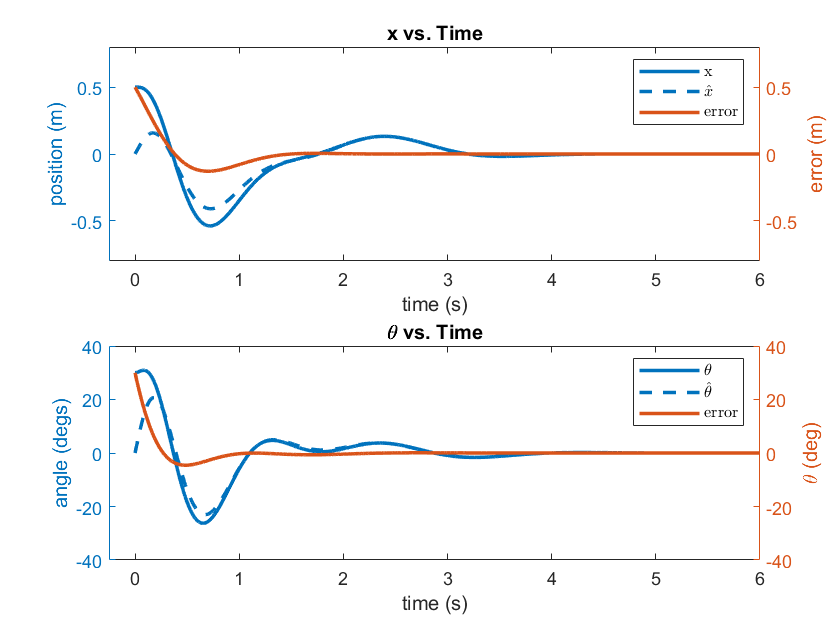
\includegraphics[width=\linewidth]{figs/p5-cl-states.png}
    \caption{Linear Model Same Poles: States \& Error vs. Time}
    \label{}
\end{figure}

\begin{figure}[!h]
    \centering
    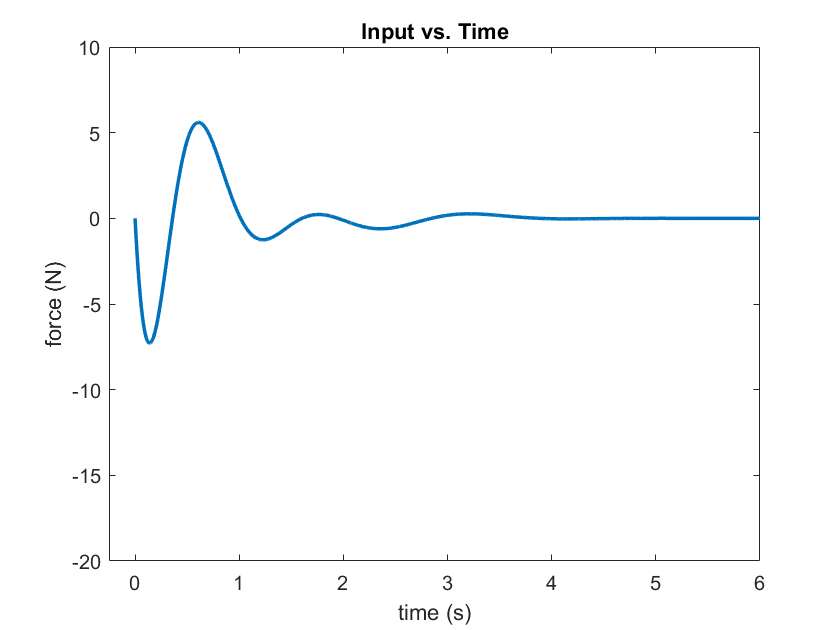
\includegraphics[width=\linewidth]{figs/p5-cl-input.png}
    \caption{Linear Model Same Poles: Control Effort vs. Time}
    \label{}
\end{figure}

\begin{figure}[!h]
    \centering
    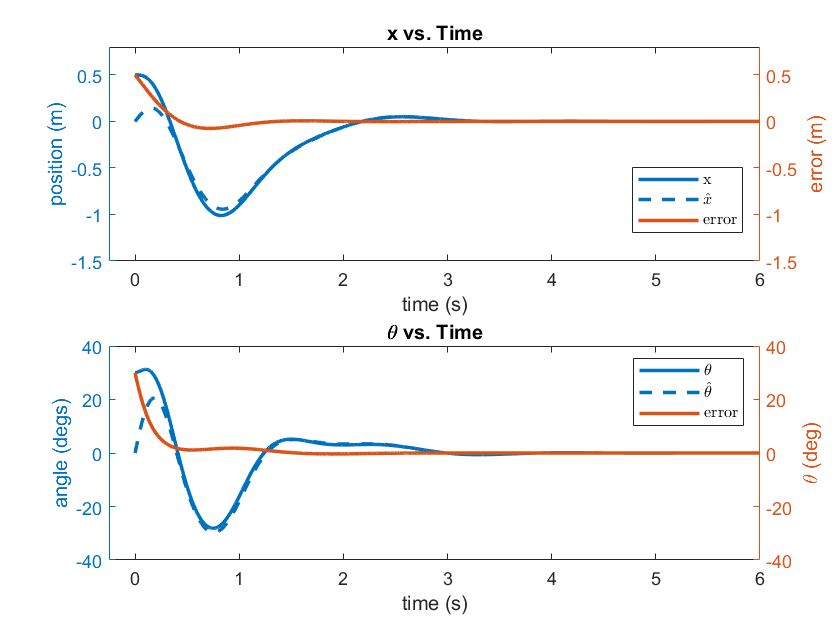
\includegraphics[width=\linewidth]{figs/p5-cnl-states.png}
    \caption{Nonlinear Model Same Poles: States \& Error vs. Time}
    \label{}
\end{figure}

\begin{figure}[!h]
    \centering
    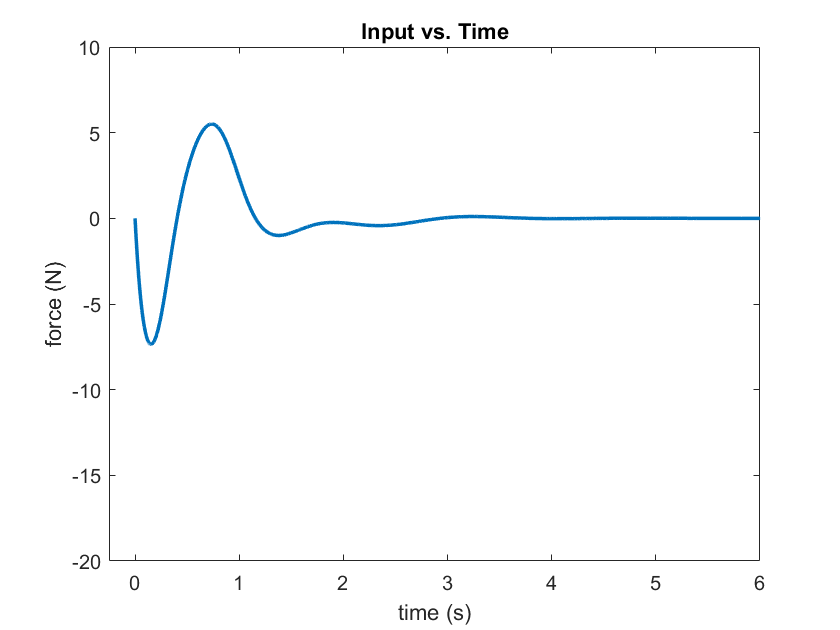
\includegraphics[width=\linewidth]{figs/p5-cnl-input.png}
    \caption{Nonlinear Model Same Poles: Control Effort vs. Time}
    \label{}
\end{figure}

\clearpage
It can be seen that the transient dynamics change completely for the case where the eigenvalues are the same for both models. However, the performance based on the design requirements is still preserved. It is still better to place the observer eigenvalues further into the left-half plane than the controller eigenvalues, but in this case, having the same eigenvalues still works.

\subsubsection*{c) Compare the responses of the state feedback and output feedback for both models.}
The outputs for each of these cases look relatively similar as there is no noise on the "measurements" we're using in our observer. The transient responses for each look slightly different on a small scale until the observer tracks with zero error; however, it is hard to notice the difference in the transients graphically. Once tracking, the responses look the same as the controller eigenvalues are the same for state and output feedback.
\clearpage

\section*{Part 6: Output Feedback Regulation (Reduced-Order)}

\subsection*{Problem 1}
The following is the derivation of the reduced order regulator:

\begin{equation*}
    \begin{split}
        T & =
        \begin{bmatrix}
            C          \\
            Invertible \\
            Invertible \\
        \end{bmatrix} \\
        & =
        \begin{bmatrix}
            1 & 0 & 0 & 0 \\
            0 & 0 & 1 & 0 \\
            0 & 1 & 0 & 0 \\
            0 & 0 & 0 & 1 \\
        \end{bmatrix}
    \end{split}
\end{equation*}

$T$ is a transformation matrix that can be used to determine a reduced order $A$ and $B$ with the following:

\begin{equation*}
    \begin{split}
        A_T & = TAT^{-1} \\
        B_T& = TB \\
    \end{split}
\end{equation*}

The observer matrix are then determined by placing the eigenvalues with the $A_{T2}$ and $A_{T4}$ sub-matrices of $A_T$. Given the system is now second order, only two eigenvalues are needed to be placed. Two of the complex conjugates previously used in Part 5.a were chosen to determine the following:

\begin{equation*}
    \begin{split}
        L & =
        \begin{bmatrix}
            17.068 & -29.394 \\
            28.939 & 17.25   \\
        \end{bmatrix}
    \end{split}
\end{equation*}

Terms of the reduced-order observer contain a derivative of the measurements (output). This can cause errors in a non-simulated system as taking the derivative of noisy measurements increases the noise. As a result, the terms of the observer are rearranged to develop a $\dot{q}$ term:

\begin{equation*}
    \begin{split}
        \dot{q} & = (A_3-LA_1)y +(A_4+LA_2)(q+Ly)+(B_2+LB_1)u
    \end{split}
\end{equation*}

$\hat{z}$ becomes the following:

\begin{equation*}
    \begin{split}
        \hat{z} & = q + Ly
    \end{split}
\end{equation*}

This means $q$ needs to be integrated in the observer Simulink block for the states to be observed. Then the $z$ states are transformed back to $x$ using $T^{-1}$ using the following:

\begin{equation*}
    \begin{split}
        \hat{x} & =
        \begin{bmatrix}
            y       \\
            \hat{z} \\
        \end{bmatrix}
    \end{split}
\end{equation*}

\clearpage

The output and input plots for the controller are shown below:

\begin{figure}[!h]
    \centering
    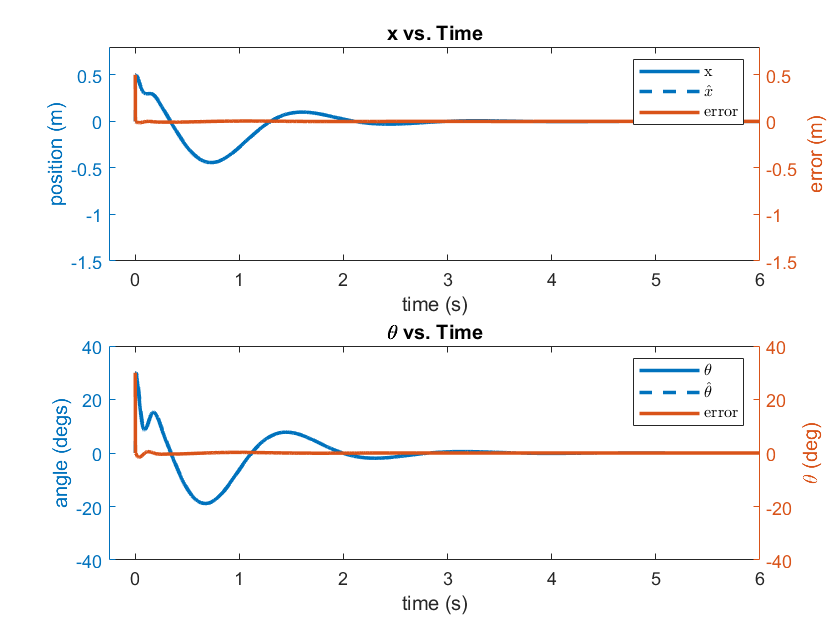
\includegraphics[width=\linewidth]{figs/p6-a-states.png}
    \caption{Nonlinear Model: States \& Error vs. Time}
    \label{}
\end{figure}

\begin{figure}[!h]
    \centering
    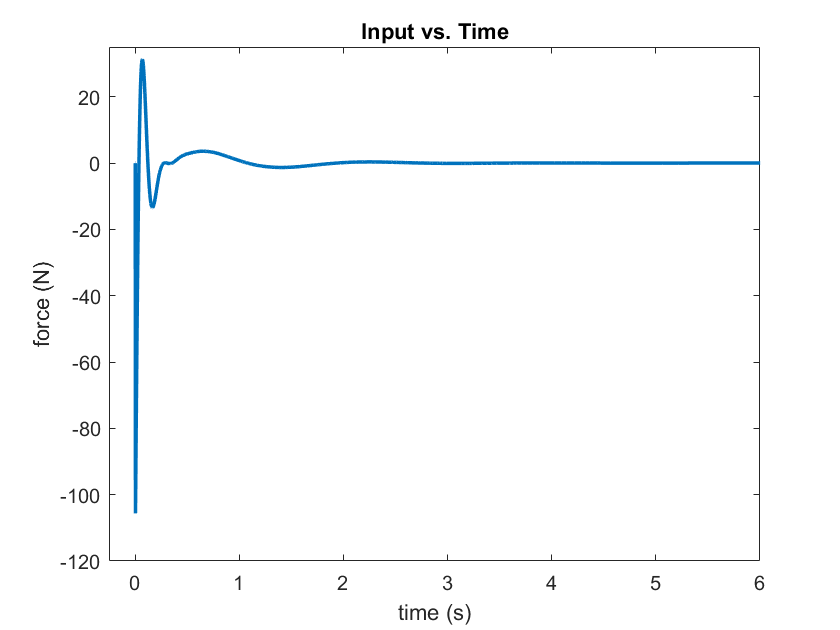
\includegraphics[width=\linewidth]{figs/p6-a-input.png}
    \caption{Nonlinear Model: Control Effort vs. Time}
    \label{}
\end{figure}

\clearpage

\subsubsection*{c) Discuss full-order and reduced-order responses.}
The reduced-order observer tracks incredibly faster using two of the same eigenvalues as the full-order observer. This is because only two states are being estimated while the others are directly measured. As a result, using the same eigenvalues is overkill and causes there to be an undesirable control effort as the eigenvalues are too far in the left half plane for the transformed system dynamics. There is too much "strain" put on the controller.


\end{document}

